\documentclass[12pt]{article}
\usepackage{fontspec}
\usepackage{xeCJK}
\setCJKmainfont[AutoFakeBold=2]{SimSun}
%\setCJKsansfont{SimHei}
\usepackage{amsmath, amssymb, amsthm}
\usepackage{geometry}
\usepackage{tikz}
\usepackage{fancyhdr}
%\setlength{\headheight}{15pt}
\usetikzlibrary{calc, intersections} % ABX 用於某些符號，若無可刪除
\usepackage{enumitem}
\usepackage{tkz-euclide}
\usepackage{subcaption}
\usepackage{float}
\usepackage[most]{tcolorbox}
\newtcolorbox{mybox}[4][證明]{
  empty,
  breakable,                % 支援跨頁
  sharp corners,
  left=#2+#3,               % 為左側標籤預留空間 (縮進)
  right=0pt, top=0pt, bottom=0pt,
  colback=white,
  % --- 加入以下這行來調整段距 ---
  before upper={\setlength{\parskip}{0.5em plus 0.2em minus 0.1em}},
  after={\vspace{#4}},
  % ---------------------------
  overlay unbroken and first={ % 在第一頁/未斷頁時繪製標籤
    \node[
      anchor=north west,
      draw, 
      inner sep=0pt,
      minimum width=#2,
      minimum height=1.6em, 
      font=\bfseries\boldmath
    ] at (frame.north west) {#1};
  }
}

\geometry{left=1.5cm, right=1.5cm, top=1.7cm, bottom=1.5cm}

% 設定頁首頁尾
\pagestyle{fancy}
\fancyhf{}
\renewcommand{\headrulewidth}{2pt}
\renewcommand{\thefigure}{圖 \thesection-\arabic{figure}} % 主圖編號
\renewcommand{\thesubfigure}{圖 \thesubsection-\arabic{subfigure}} % 子圖變為 2-1
\captionsetup[figure]{labelformat=simple, labelsep=quad} 
\captionsetup[subfigure]{labelformat=simple} % 移除括號
\lhead{廖汶鋒}
\chead{四點共圓}
\rhead{澳門培道中學}
\fancyfoot[C]{\thepage} % Centered footer
%\fancyfoot[L]{2026年2月7日} % Left footer

%\title{四點共圓}
%\author{廖汶鋒}
%\date{2026年2月7日}
\linespread{1.3}

% 定段落首行縮進（兩個中文字）
\setlength{\parindent}{2em}
\setlength{\headheight}{15pt} % 避免頁首高度警告
\begin{document}
\thispagestyle{fancy}  % 讓首頁也顯示頁首
%\maketitle
\begin{center}
    \textbf{\Large{四點共圓}}
\end{center}
四點共圓是競賽幾何題中的一個至關重要題種，是指不共線的四點位於同一圓上。
目前我們知道「任意不共線三點，有且只有一個通過此三點的圓」，但任意四點是否共圓則需要進一步判斷。
大部分讀者存在「幾何恐懼」的現象，就是因為沒有掌握好處理這類題目的方法。
本文將介紹多種常見的方法來處理四點共圓問題，並通過例題來說明這些方法的應用。

\section{與弦、弧、角相關的性質}
\begin{mybox}[垂徑定理]{6em}{1em}{0.5em}
    垂直於弦的直徑平分弦，並且平分弦所對的優弧及劣弧。
\end{mybox}
\begin{mybox}[圓周角定理]{7em}{1em}{0.5em}
    \begin{enumerate}[label= \arabic*., itemsep=0.2em]
        \item 同弧或等弧所對的圓周角是圓心角的一半；
        \item 同弦且分佈在弦的同側的圓周角相等；
        \item 同弦且分佈在弦的異側的圓周角互補。
    \end{enumerate}
\end{mybox}
\begin{mybox}[圓冪定理]{6em}{1em}{0.5em}
    圓$\Gamma$上存在四個不同點$A$、$B$、$C$、$D$，設直線$AB$與直線$CD$交於點$P$，
    則有$\overrightarrow{PA}\cdot\overrightarrow{PB}=\overrightarrow{PC}\cdot\overrightarrow{PD}$。
    \begin{enumerate}[label= \arabic*., itemsep=0.2em]
        \item 相交弦定理；
        \item 兩割線定理；
        \item 切割線定理。
    \end{enumerate}
\end{mybox}
\begin{mybox}[弦切角定理]{7em}{1em}{0.5em}
    圓$\Gamma$上存在兩個不同點$A$、$B$，設直線$PB$與圓$\Gamma$相切，那麼任取圓$\Gamma$上且不在$\angle{PBA}$內部的一點$C$，都有$\angle{PBA}=\angle{BCA}$。
\end{mybox}
\newpage
\section{四點共圓常用判定方法}
\subsection{圓的定義}
\begin{mybox}[定理]{4em}{1em}{1em}
    $A$、$B$、$C$、$D$四點共圓的充分必要條件是存在一點$O$使得$OA=OB=OC=OD$。
\end{mybox}
\subsection{圓周角}
\begin{mybox}[定理]{4em}{1em}{0.5em}
    對於不共線的四點$A$、$B$、$C$、$D$
    \begin{enumerate}[itemsep=0.3em]
        \item 若$B$、$D$同時位於直線$AC$的同側，則$A$、$B$、$C$、$D$四點共圓的充分必要條件是$\angle{ABC}=\angle{ADC}$；
        \item 若$B$、$D$分別位於直線$AC$的異側，則$A$、$B$、$C$、$D$四點共圓的充分必要條件是$\angle{ABC}+\angle{ADC}=180^\circ$。
    \end{enumerate}
    \begin{figure}[H]
        \centering
        \begin{subfigure}[b]{0.45\textwidth}
            \centering
            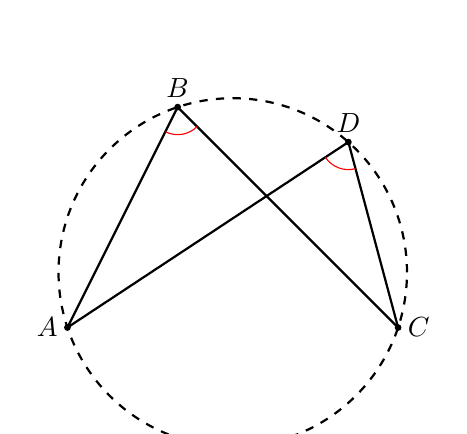
\begin{tikzpicture}[scale=0.7]
                \tkzDefPoint(0,4){B}
                \tkzDefPoint(-2,0){A}
                \tkzDefPoint(4,0){C}
                \tkzCircumCenter(A,B,C) \tkzGetPoint{O}
                \tkzDefPointBy[rotation=center O angle -60](B) \tkzGetPoint{D}
                \tkzDrawCircle[black, thick, dashed](O,B)
                \tkzDrawPoints[fill=black](A,B,C,D)
                \tkzDrawSegments[black, thick](A,B B,C A,D D,C)
                \tkzLabelPoints[above](B,D)
                \tkzLabelPoints[left](A)
                \tkzLabelPoints[right](C)
                \tkzMarkAngle[color=red, size=0.5](A,B,C)
                \tkzMarkAngle[color=red, size=0.5](A,D,C)
            \end{tikzpicture}
            \caption{$B$、$D$同時位於直線$AC$的同側}
            \label{fig:concyclic_s2.1-1}
        \end{subfigure}
        \hfill % 在兩圖之間加入彈性間距
        \begin{subfigure}[b]{0.45\textwidth}
            \centering
            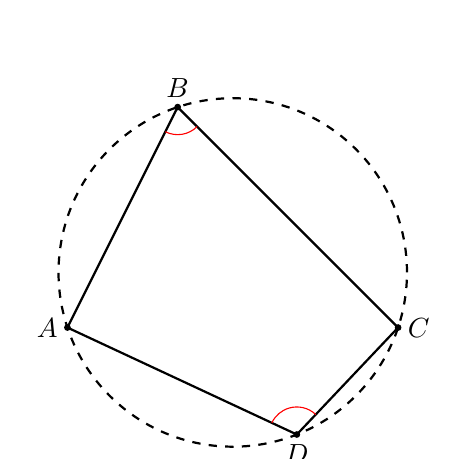
\begin{tikzpicture}[scale=0.7]
                \tkzDefPoint(0,4){B}
                \tkzDefPoint(-2,0){A}
                \tkzDefPoint(4,0){C}
                \tkzCircumCenter(A,B,C) \tkzGetPoint{O}
                \tkzDefPointBy[rotation=center O angle -50](C) \tkzGetPoint{D}
                \tkzDrawCircle[black, thick, dashed](O,B)
                \tkzDrawPoints[fill=black](A,B,C,D)
                \tkzDrawSegments[black, thick](A,B B,C A,D D,C)
                \tkzLabelPoints[left](A)
                \tkzLabelPoints[above](B)
                \tkzLabelPoints[right](C)
                \tkzLabelPoints[below](D)
                \tkzMarkAngle[color=red, size=0.5](A,B,C)
                \tkzMarkAngle[color=red, size=0.5](C,D,A)
            \end{tikzpicture}
            \caption{$B$、$D$分別位於直線$AC$的異側}
            \label{fig:concyclic_s2.1-2}
        \end{subfigure}
    \end{figure}
\end{mybox}
\begin{mybox}[例題\thesubsection-1]{6em}{1em}{0.5em}
    在$\triangle{ABC}$中，$D$和$E$分別是$AB$和$AC$上的點，滿足$CD\perp AB$和$BE\perp AC$。記$CD$與$BE$的交點為$H$，求證：
    \begin{enumerate}[label = (\roman*.), itemsep=0.3em]
        \item $B$、$C$、$D$、$E$四點共圓；
        \item $A$、$D$、$E$、$H$四點共圓。
    \end{enumerate}
\end{mybox}
\begin{mybox}[例題\thesubsection-2]{6em}{1em}{0.5em}
    在$\triangle{ABC}$中，$D$和$E$分別是線段$AB$和$AC$上的點，滿足$\triangle{AED}\sim\triangle{ABC}$。

    求證：$B$、$C$、$D$、$E$四點共圓。
\end{mybox}
\begin{mybox}[例題\thesubsection-3]{6em}{1em}{1em}
    對於銳角$\triangle{ABC}$，記$H$為$\triangle{ABC}$的垂心，$H_A$、$H_B$、$H_C$分別為$H$關於$BC$、$CA$、$AB$的對稱點。
    求證：$A$、$B$、$C$、$H_A$、$H_B$、$H_C$六點共圓。
\end{mybox}
\iffalse
\begin{center}
    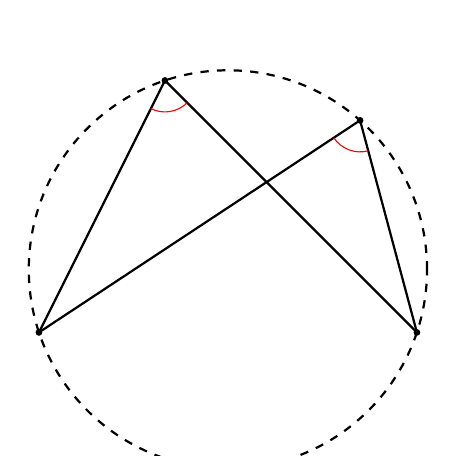
\begin{tikzpicture}[scale=0.8]
        \tkzDefPoint(0,4){B}
        \tkzDefPoint(-2,0){A}
        \tkzDefPoint(4,0){C}
        \tkzCircumCenter(A,B,C) \tkzGetPoint{O}
        \tkzDefPointBy[rotation=center O angle -60](B) \tkzGetPoint{D}
        \tkzDrawCircle[black, thick, dashed](O,B)
        \tkzDrawPoints[fill=black](A,B,C,D)
        \tkzDrawSegments[black, thick](A,B B,C A,D D,C)
        \tkzMarkAngle[color=red, size=0.5](A,B,C)
        \tkzMarkAngle[color=red, size=0.5](A,D,C)
    \end{tikzpicture}
    \hspace{1cm}
    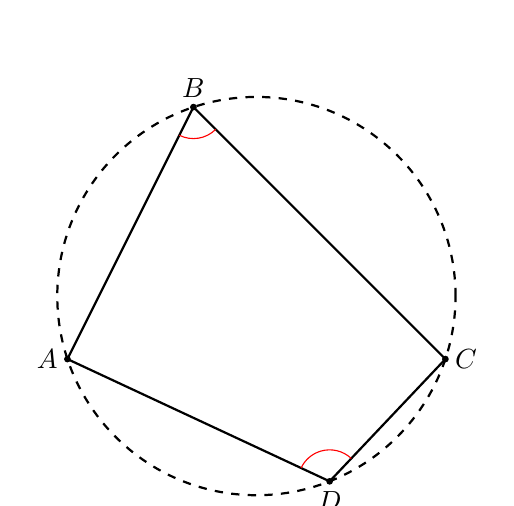
\begin{tikzpicture}[scale=0.8]
        \tkzDefPoint(0,4){B}
        \tkzDefPoint(-2,0){A}
        \tkzDefPoint(4,0){C}
        \tkzCircumCenter(A,B,C) \tkzGetPoint{O}
        \tkzDefPointBy[rotation=center O angle -50](C) \tkzGetPoint{D}
        \tkzDrawCircle[black, thick, dashed](O,B)
        \tkzDrawPoints[fill=black](A,B,C,D)
        \tkzDrawSegments[black, thick](A,B B,C A,D D,C)
        \tkzLabelPoints[left](A)
        \tkzLabelPoints[above](B)
        \tkzLabelPoints[right](C)
        \tkzLabelPoints[below](D)
        \tkzMarkAngle[color=red, size=0.5](A,B,C)
        \tkzMarkAngle[color=red, size=0.5](C,D,A)
    \end{tikzpicture}
    \vspace{0.5cm}
    \noindent
    \begin{minipage}{0.5\textwidth}
        \centering
        圖2-1\quad $B$、$D$同時位於直線$AC$的同側
    \end{minipage}%
    \begin{minipage}{0.5\textwidth}
        \centering
        圖2-2\quad $B$、$D$分別位於直線$AC$的異側
    \end{minipage}
\end{center}
\fi
\subsection{圓冪}
\begin{mybox}[定理]{4em}{1em}{1em}
    對於不共線的四點$A$、$B$、$C$、$D$，設直線$AB$與直線$CD$交於點$P$，
    則$A$、$B$、$C$、$D$四點共圓的充分必要條件是
    $$\overrightarrow{PA}\cdot\overrightarrow{PB}=\overrightarrow{PC}\cdot\overrightarrow{PD}$$
    \begin{enumerate}[label = \arabic*., itemsep=0.3em]
        \item 相交弦定理；
        \item 兩割線定理。
    \end{enumerate}
    \begin{figure}[H]
        \centering
        \begin{subfigure}[b]{0.45\textwidth}
            \centering
            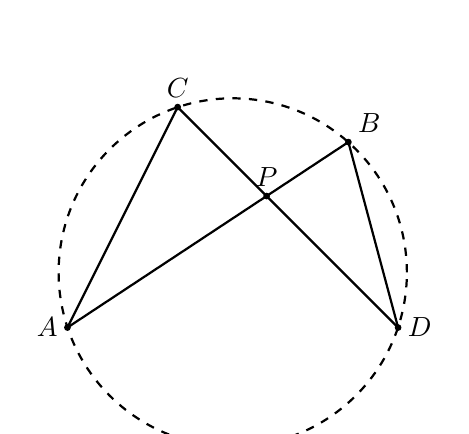
\begin{tikzpicture}[scale=0.7]
                \tkzDefPoint(0,4){C}
                \tkzDefPoint(-2,0){A}
                \tkzDefPoint(4,0){D}
                \tkzCircumCenter(C,A,D) \tkzGetPoint{O}
                \tkzDefPointBy[rotation=center O angle -60](C) \tkzGetPoint{B}
                \tkzDrawCircle[black, thick, dashed](O,B)
                \tkzInterLL(A,B)(C,D) \tkzGetPoint{P}
                \tkzDrawPoints[fill=black](A,B,C,D,P)
                \tkzDrawSegments[black, thick](A,B C,D A,C B,D)
                \tkzLabelPoints[left](A)
                \tkzLabelPoints[above](C,P)
                \tkzLabelPoints[right](D)
                \tkzLabelPoints[above right](B)
            \end{tikzpicture}
            \caption{相交弦定理}
            \label{fig:concyclic_s2.2-1}
        \end{subfigure}
        \hfill % 在兩圖之間加入彈性間距
        \begin{subfigure}[b]{0.45\textwidth}
            \centering
            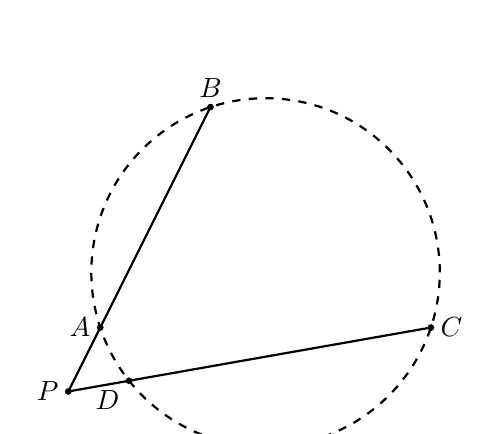
\begin{tikzpicture}[scale=0.7]
                \tkzDefPoint(0,4){B}
                \tkzDefPoint(-2,0){A}
                \tkzDefPoint(4,0){C}
                \tkzCircumCenter(A,B,C) \tkzGetPoint{O}
                \tkzDefPointBy[rotation=center O angle 20](A) \tkzGetPoint{D}
                \tkzDrawCircle[black, thick, dashed](O,B)
                \tkzInterLL(A,B)(C,D) \tkzGetPoint{P}
                \tkzDrawPoints[fill=black](A,B,C,D,P)
                \tkzDrawSegments[black, thick](P,B P,C)
                \tkzLabelPoints[left](A)
                \tkzLabelPoints[above](B)
                \tkzLabelPoints[right](C)
                \tkzLabelPoints[below left](D)
                \tkzLabelPoints[left](P)
            \end{tikzpicture}
            \caption{兩割線定理}
            \label{fig:concyclic_s2.2-2}
        \end{subfigure}
    \end{figure}
\end{mybox}
\begin{mybox}[例題\thesubsection-1]{6em}{1em}{1em}
    圓$\Omega$和圓$\Gamma$相交於點$A$和$B$。在直線$BA$的延長線上任取一點$K$，
    過$K$點作直線$l_1$交圓$\Omega$於點$C$和$D$，作直線$l_2\neq l_1$交圓$\Omega$於點$E$和$F$。
    
    求證：$C$、$D$、$E$、$F$四點共圓。
\end{mybox}
\iffalse
\begin{mybox}[證明]{4em}{1em}{1em}
    我們只需證明$A$、$B$、$C$、$H_A$四點共圓，因為其餘兩組點的證明方法類似。\\

    方法一：圓周角定理
    
    由於$H$為$\triangle{ABC}$的垂心，故有
    \begin{equation}
        \begin{cases}
            \angle{CBH} = 90^\circ - \angle{ACB}, \\
            \angle{BCH} = 90^\circ - \angle{ABC}
        \end{cases}
    \end{equation}
    所以
    \begin{align}
        \angle{BHC}&=180^\circ-\angle{CBH}-\angle{BCH}\notag\\
        &=180^\circ-(90^\circ-\angle{ACB})-(90^\circ-\angle{ABC})\notag\\
        &=\angle{ABC}+\angle{ACB}\notag\\
        &=180^\circ-\angle{BAC}
    \end{align}
    又因為$H_A$為$H$關於$BC$的對稱點，故有
    \begin{equation}
        \angle{BH_AC}=\angle{BHC}=180^\circ-\angle{BAC}
    \end{equation}
    由圓周角定理可知，$A$、$B$、$C$、$H_A$四點共圓。  
    
    同理可得，$A$、$B$、$C$、$H_A$、$H_B$、$H_C$六點共圓。
\end{mybox}
\fi
\begin{mybox}[例題\thesubsection-2]{6em}{1em}{1em}
    同一個平面內有兩條不重合且不平行的直線$l_1$和$l_2$，
    點$A$、$B$、$C$是直線$l_1$上的三個相異點，點$D$、$E$和$F$是直線$l_2$上的三個相異點。
    已知$A$、$B$、$D$、$E$四點共圓，$AD\parallel CF$。求證：$B$、$C$、$E$、$F$四點共圓。
\end{mybox}
\iffalse
\begin{mybox}[證明]{4em}{1em}{1em}
    由圓冪定理可知
    \begin{equation}
        \overrightarrow{KC}\cdot\overrightarrow{KD}=\overrightarrow{KA}\cdot\overrightarrow{KB}=\overrightarrow{KE}\cdot\overrightarrow{KF}
    \end{equation}
    所以$C$、$D$、$E$、$F$四點共圓。
\end{mybox}
\fi
\newpage
\subsection{托勒密定理}
本節主要介紹托勒密定理的判定方法，首先引用更強的托勒密不等式。
\begin{mybox}[托勒密不等式]{8em}{1em}{1em}
    對於凸四邊形$ABCD$，都有
    $$AB \cdot CD + AD \cdot BC \geq AC \cdot BD$$
    等號成立當且僅當$A$、$B$、$C$、$D$四點共圓。
\end{mybox}
\begin{mybox}[證明]{4em}{1em}{1em}
    \begin{figure}[H]
        \centering
        \begin{subfigure}[b]{\textwidth}
            \centering
            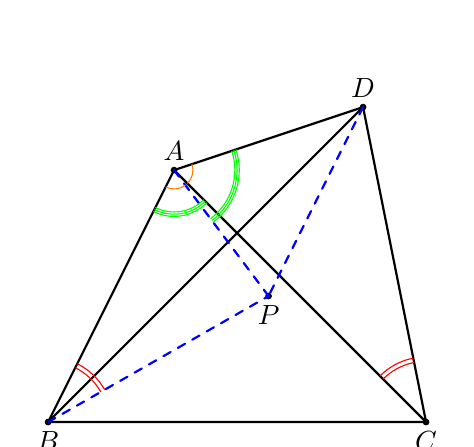
\begin{tikzpicture}[scale=0.8]
                \tkzDefPoint(0,4){A}
                \tkzDefPoint(-2,0){B}
                \tkzDefPoint(4,0){C}
                \tkzDefPoint(3,5){D}
                \tkzFindAngle(C,A,D) \tkzGetAngle{CAD}
                \tkzFindAngle(D,C,A) \tkzGetAngle{DCA}
                \tkzDefPointBy[rotation=center A angle \CAD](B) \tkzGetPoint{B_tmp}
                \tkzDefPointBy[rotation=center B angle -\DCA](A) \tkzGetPoint{A_tmp}
                \tkzInterLL(A,B_tmp)(B,A_tmp) \tkzGetPoint{P}
                \tkzDrawPolygon[black, thick](A,B,C,D)
                \tkzDrawPoints[fill=black](A,B,C,D,P)
                \tkzDrawSegments[black, thick](A,C B,D)
                \tkzDrawSegments[blue, thick, dashed](A,P B,P D,P)
                \tkzLabelPoints[above](A,D)
                \tkzLabelPoints[below](B,C,P)
                \tkzMarkAngle[size=0.3, color=orange, fill=orange!30](B,A,P)
                \tkzMarkAngle[size=0.3, color=orange, fill=orange!30](C,A,D)
                \tkzMarkAngle[color=red, arc=ll, fill=red!30](P,B,A)
                \tkzMarkAngle[color=red, arc=ll, fill=red!30](D,C,A)
                \tkzMarkAngle[size=0.7, color=green, arc=lll, fill=green!30](B,A,C)
                \tkzMarkAngle[color=green, arc=lll, fill=green!30](P,A,D)
            \end{tikzpicture}
            \caption{托勒密不等式示意圖}
            \label{fig:concyclic_s2.3-1}
        \end{subfigure}
    \end{figure}
    作直線$l_1$，使$\measuredangle{\left(AB,l_1\right)}=\measuredangle{CAD}$；
    
    作直線$l_2$，使$\measuredangle{\left(BA,l_2\right)}=\measuredangle{ACD}$。

    設$l_1$與$l_2$交於點$P$，則有$\triangle{APB}\sim\triangle{ADC}$，所以
    \begin{equation}
        \frac{AP}{AD}=\frac{AB}{AC}=\frac{PB}{DC} \Rightarrow AB\cdot CD=AC\cdot BP\label{eq:ptolemy_ineq_1}
    \end{equation}
    同時亦能注意到$\triangle{ABC}\sim\triangle{APD}$，所以
    \begin{equation}
       \frac{AC}{AD}=\frac{BC}{PD} \Rightarrow AD\cdot BC=AP\cdot DP\label{eq:ptolemy_ineq_2}
    \end{equation}
    把\eqref{eq:ptolemy_ineq_1}和\eqref{eq:ptolemy_ineq_2}相加，得到
    \begin{equation}
        AB\cdot CD + AD\cdot BC = AC\cdot\left(BP + DP\right)\geq AC\cdot BD\label{eq:ptolemy_ineq_3}
    \end{equation}
    等號成立條件為$P$位於線段$BD$上，即等價於
    $$\measuredangle{ACD}=\measuredangle{ABP}=\measuredangle{ABD}\Leftrightarrow \text{$A$、$B$、$C$、$D$四點共圓}$$
\end{mybox}
\begin{mybox}[托勒密定理]{7em}{1em}{1em}
    對於凸四邊形$ABCD$，$A$、$B$、$C$、$D$四點共圓的充分必要條件是
    $$AB \cdot CD + AD \cdot BC = AC \cdot BD$$
\end{mybox}
\subsection{三弦定理}
\begin{mybox}[定理]{4em}{1em}{1em}
    對於凸四邊形$ABCD$，$A$、$B$、$C$、$D$四點共圓的充分必要條件是
    $$AB\sin{\angle{DAC}} + AD\sin{\angle{CAB}} = AC\sin{\angle{DAB}}$$
    \begin{figure}[H]
        \centering
        \begin{subfigure}[b]{\textwidth}
            \centering
            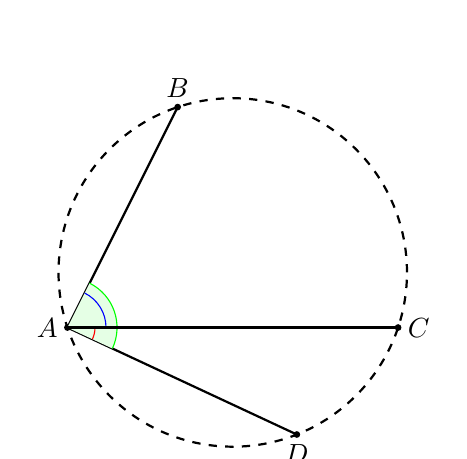
\begin{tikzpicture}[scale=0.7]
                \tkzDefPoint(0,4){B}
                \tkzDefPoint(-2,0){A}
                \tkzDefPoint(4,0){C}
                \tkzCircumCenter(A,B,C) \tkzGetPoint{O}
                \tkzDefPointBy[rotation=center O angle -50](C) \tkzGetPoint{D}
                \tkzDrawCircle[black, thick, dashed](O,B)
                \tkzDrawPoints[fill=black](A,B,C,D)
                \tkzDrawSegments[black, thick](A,B A,D)
                \tkzLabelPoints[left](A)
                \tkzLabelPoints[above](B)
                \tkzLabelPoints[right](C)
                \tkzLabelPoints[below](D)
                \tkzFillAngle[fill=green!10, size=0.9](D,A,B)
                \tkzMarkAngle[color=red, size=0.5](D,A,C)
                \tkzMarkAngle[color=blue, size=0.7](C,A,B)
                \tkzMarkAngle[color=green, size=0.9](D,A,B)
                \tkzDrawSegment[black, thick](A,C)
            \end{tikzpicture}
            \caption{三弦定理的示意圖}
            \label{fig:concyclic_s2.4-1}
        \end{subfigure}
    \end{figure}
\end{mybox}
\begin{mybox}[思考]{4em}{1em}{1em}
    換成有向角（例：$\angle{DAC}\rightarrow\measuredangle{DAC}$）是否依然成立？
\end{mybox}
\begin{mybox}[例題\thesubsection-1]{6em}{1em}{1em}
    $\triangle{ABC}$的內心和$A$點所對旁心分別為$I$和$J_A$，$I$和$J_A$分在直線$AB$上的投影分別為$E$和$F$，$E$關於$A$的對稱點為$E'$。
    現射線$AI$上存在一點$D$，其在$AB$上的投影為$D'$。如果$2AD'=E'F$，求證：$A$、$B$、$C$、$D$四點共圓。
\end{mybox}
\section{與三點共線的聯繫}
\begin{mybox}[西姆松定理]{7em}{1em}{1em}
    同一平面上已知$\triangle{ABC}$以及$\triangle{ABC}$外一點$P$，$P$分別在直線$BC$、$CA$和$AB$上的投影分別為$D$、$E$和$F$。
    那麼，$A$、$B$、$C$、$P$四點共圓的充分必要條件是$D$、$E$、$F$三點共線。
\end{mybox}
\section{與三線共點的聯繫}
\begin{mybox}[根軸]{4em}{1em}{1em}
    對於兩個非同心圓$\odot{O_1}$和$\odot{O_2}$，其半徑分別為$R_1$和$R_2$。由$\odot{O_1}$和$\odot{O_2}$誘導出來的「根軸」$l_{12}$是指
    $$
        l_{12}=\left\{P\text{是動點}\ |\ O_1P^2-R_1^2=O_2P^2-R_2^2\right\}
    $$
\end{mybox}
\begin{mybox}[定理1]{4em}{1em}{1em}
    根軸是一條垂直於連心線$O_1O_2$的直線。
\end{mybox}
\begin{mybox}[定理2]{4em}{1em}{1em}
    兩圓外切，根軸為內公切線；兩圓相交，根軸為兩個交點連成的直線；兩圓內切，根軸為外公切線。
\end{mybox}
\begin{mybox}[定理3]{4em}{1em}{1em}
    對於三個圓心不共線的圓$\odot{O_1}$、$\odot{O_2}$和$\odot{O_3}$，根軸$l_{12}$、$l_{23}$、$l_{31}$三線共點。交點稱為「根心」。
\end{mybox}
\begin{mybox}[例題\thesection-1]{6em}{1em}{1em}
    已知$BCDE$是圓內接四邊形，$A$是$BCDE$外接圓外的一點。
    若$BC$交$DE$於$P$，$AP$交$\triangle{ADE}$的外接圓於$K$點，則$A$、$B$、$C$、$K$四點共圓。
\end{mybox}
\section{練習題}
\begin{mybox}[Problem 1]{7em}{1em}{1em}
   對於$\triangle{ABC}$，記$I$為$\triangle{ABC}$的內心，$J_A$為$\angle{CBA}$和$\angle{BCA}$的外角平分線的交點。

   求證：$B$、$I$、$J_A$、$C$四點共圓。
\end{mybox}
\begin{mybox}[Problem 2]{7em}{1em}{1em}
   承上題，記$IJ_A$的中點$D_A$。
   
   求證：$A$、$B$、$C$、$D_A$四點共圓且$A$、$I$、$D_A$、$J_A$四點共線。
\end{mybox}
\begin{mybox}[Problem 3]{7em}{1em}{1em}
    對於鈍角$\triangle{ABC}$，記$H$為$\triangle{ABC}$的垂心，$H_A$、$H_B$、$H_C$分別為$H$關於$BC$、$CA$、$AB$的對稱點。
    求證：$A$、$B$、$C$、$H_A$、$H_B$、$H_C$六點共圓。
\end{mybox}
\begin{mybox}[Problem 4*]{7em}{1em}{1em}
    令$H$是銳角$\triangle{ABC}$的垂心，$F$是$C$在$AB$邊上的投影，$P$是$H$關於$BC$的對稱點。
    假設$\triangle{AFP}$的外接圓交直線$BC$於$X$和$Y$兩個相異點，求證：$C$是線段$XY$的中點。
\end{mybox}
\begin{mybox}[Problem 5*]{7em}{1em}{1em}
   如下圖，在四邊形$ABCD$中，$AB=AD$，$CB=CD$，$\angle{ABC}=90^\circ$。點$E$和$F$分別在線段$AB$和$AD$上，點$P$和$Q$在線段$EF$上（$P$在$E$和$Q$之間），\
   滿足$AE:EP=AF:FQ$。點$X$和$Y$分別在線段$CP$和$CQ$上，滿足$BX\perp CP$及$BY\perp CQ$。
   
   求證：$X$、$Y$、$P$、$Q$四點共圓。 
   \begin{center}
    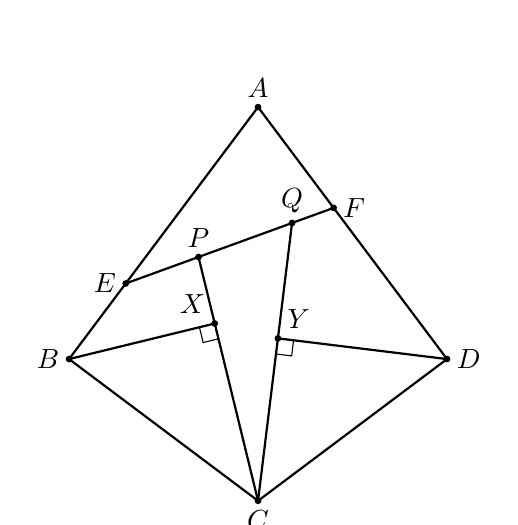
\begin{tikzpicture}[scale=1]
        \tkzDefPoints{0/0/A, -2.4/-3.2/B, 0/-5/C, 2.4/-3.2/D}
        \coordinate (E) at ($(A)!0.7!(B)$);
        \coordinate (F) at ($(A)!0.4!(D)$);
        \coordinate (P) at ($(E)!0.35!(F)$);
        \coordinate (Q) at ($(F)!0.2!(E)$);
        \tkzDefPointBy[projection=onto C--P](B) \tkzGetPoint{X}
        \tkzDefPointBy[projection=onto C--Q](D) \tkzGetPoint{Y}
        \tkzDrawPoints[fill=black](A,B,C,D,E,F,P,Q,X,Y)
        \tkzDrawPolygon[black, thick](A,B,C,D)
        \tkzDrawSegments[black, thick](E,F C,P C,Q B,X D,Y)
        \tkzLabelPoints[above](A,P,Q)
        \tkzLabelPoints[left](B,E)
        \tkzLabelPoints[right](D,F)
        \tkzLabelPoints[below](C)
        \tkzLabelPoints[above left](X)
        \tkzLabelPoints[above right](Y)
        \tkzMarkRightAngle[size=0.2](B,X,C)
        \tkzMarkRightAngle[size=0.2](C,Y,D)
    \end{tikzpicture}
   \end{center}
\end{mybox}
\begin{mybox}[Problem 6]{7em}{1em}{1em}
    $AP$是$\triangle{ABC}$中的邊$BC$上的陪位中線，$D$、$E$分別在直線$AB$、$AC$上，$AP$平分線段$DE$，

    求證：$B$、$C$、$D$、$E$四點共圓。
\end{mybox}
\begin{mybox}[Problem 7]{7em}{1em}{1em}
    直線$l_1$上依次排列着$B_1$、$C_1$、$D_1$四點，直線$l_2$上依次排列着$B_2$、$C_2$、$D_2$四點。
    若$B_1B_2C_2C_1$和$C_1C_2D_2D_1$都是圓內接四邊形，

    求證：$B_1B_2\parallel D_1D_2$。
\end{mybox}
\end{document}